% arara: pdflatex: { interaction: nonstopmode }
% arara: biber
% arara: pdflatex: { interaction: nonstopmode }
% % arara: pdflatex: { interaction: nonstopmode }
% arara: clean: { extensions: [ log, aux, synctex ] }

\documentclass[aspectratio=169]{beamer}

\usepackage[utf8]{inputenc}
\usepackage{mathrsfs}
\usepackage[style=verbose,backend=biber]{biblatex}
\usepackage{tabularx}
\addbibresource{../master_thesis.bib}

\AtEveryCitekey{
	\clearfield{urlday}
	\clearfield{urlyear}
	\clearfield{urlmonth}
	\clearfield{urldate}
	\clearfield{timestamp}
	\clearfield{year}
	\clearlist{institution}
	\clearfield{type}
}
		

\usetheme{Boadilla}

\setbeamertemplate{navigation symbols}{}

\title[Master's Thesis Kick-Off]{Adopting Random Slicing as the Partitioning Algorithm in Riak Core Lite}
\subtitle{Master's Thesis Kick-Off}
\author{Pascal Grosch}
\institute{TU Kaiserslautern}
\date{July 1, 2020}

\graphicspath{{../images/}}

\begin{document}
\frame{\titlepage}
\section{Introduction}
\begin{frame}
\frametitle{Introduction}
\begin{itemize}
\item Riak is a distributed key-value-store
\item Based on Amazon Dynamo
\item Riak Core is a library for distributed platforms
\item Riak Core Lite was forked to create a minimal up-to-date version
\end{itemize}
\end{frame}

\section{Riak Core's Consistent Hashing}
\begin{frame}
\frametitle{Riak Core's Consistent Hashing}
\begin{itemize}
\item Based on Amazon Dynamo
\item Visual representation as a partitioned ring
\item Each partition virtual node
\item Multiple vnodes per physical nodes
\item bucket and index hashed with SHA-1 to partition index
\item Entry replicated on N neighboring partitions
\item Retrieval via hashing bucket and index and looking up N neighboring partitions
\item Retrieval successful if at least R lookups are successful
\end{itemize}
\end{frame}

\begin{frame}
\frametitle{Consistent Hashing - Visual Representation}
\begin{figure}
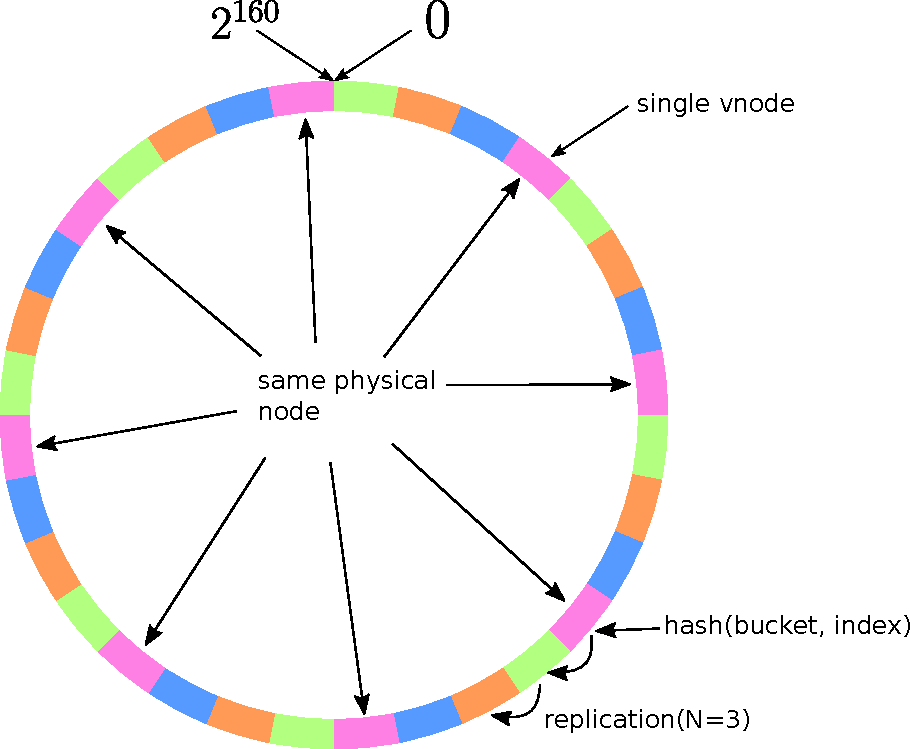
\includegraphics[height=0.8\textheight]{../images/chash_description}
\end{figure}
\end{frame}

\begin{frame}
\frametitle{Consistent Hashing - Retrieval}
\begin{figure}
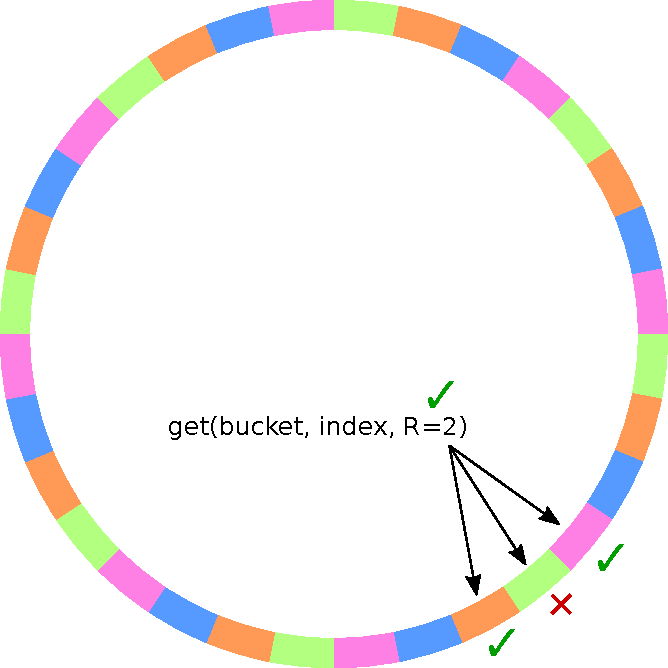
\includegraphics[height=0.8\textheight]{chash_retrieval}
\end{figure}
\end{frame}

\begin{frame}
\frametitle{Constraints}
As pointed out by Scott Lystig Fritchie\footnote{https://www.infoq.com/articles/dynamo-riak-random-slicing/}
\begin{itemize}
\item SHA-1 only feasible hash algorithm
\item 160-Bit output sets range as $0$ to $2^{160}-1$
\item Partition number is fixed at initialization
\item Number of Partitions has to be power of 2
\item Partition sized is fixed
\item Claim assignment algorithm can lead to unbalanced workload
\item No weighting of nodes with different capacities
\item No ``Justin Bieber's Twitter'' handling
\item Unchangeable replica placement policy
\end{itemize}
\end{frame}

\section{Random Slicing}
\begin{frame}
\frametitle{Random Slicing}
\begin{itemize}
\item Alternative randomized data-distribution strategy
\item Partitions $[0,1)$ range to buckets
\item Hash function to real number in $[0,1)$
\item Multiple buckets can be handled by the same node
\end{itemize}
\end{frame}

\begin{frame}
\frametitle{Random Slicing}
\begin{figure}
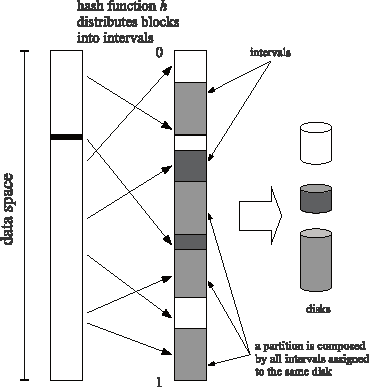
\includegraphics[height=0.8\textheight]{rslicing_description}
\caption{\protect\cite{Miranda2014}}
\end{figure}
\end{frame}

\begin{frame}
\frametitle{Changing Nodes}
\begin{itemize}
\item On adding or removing nodes the new relative capacity of remaining nodes is computed
\item Gaps are created by an algorithm and are assigned to new partitions
\begin{itemize}
\item If necessary, existing partitions are split up and moved to gaps
\item Trade-off between computing new partition intervals and moving data
\end{itemize}
\end{itemize}
\begin{figure}
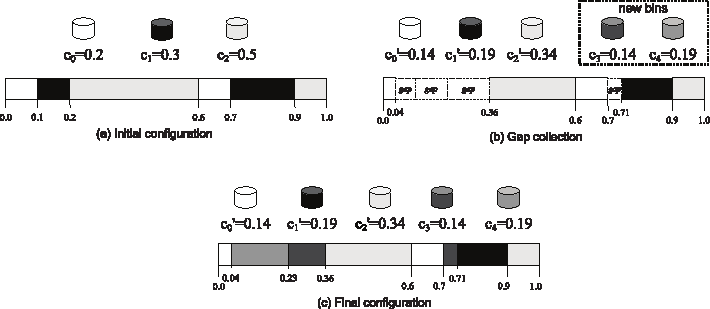
\includegraphics[height=0.5\textheight]{rslicing_gap_collection}
\caption{\protect\cite{Miranda2014}}
\end{figure}
\end{frame}

\begin{frame}
\frametitle{Performance Comparison}
\begin{table}
\begin{tabularx}{\textwidth}{|l|X|X|X|}
\hline
 & Consistent Hashing (fixed) & Consistent Hashing (adapt.) & Random Slicing\\\hline\hline
 Fairness & Poor ($\delta\uparrow$ with $n$) & Moderate ($\delta\approx10\%$) & Good ($\delta\approx 0.4\%$)\\\hline
 Memory Usage & High ($\mu\approx800$MB) & High ($\mu\approx8$GB) & Low ($\mu\approx4.5$MB)\\\hline
 Lookup Time & Moderate ($r\approx50\mu s$) & High ($r\approx98\mu s$) & Low ($r\approx14\mu s$)\\\hline
 Adaptativity & Good ($\alpha\approx7\%$) & Poor ($\alpha\approx1172\%$) & Good ($\alpha\approx1.63\%$)\\\hline
\end{tabularx}
\caption{\emph{Definitions used}: $n$, number of devices; $\delta$, average deviation from ideal load; $\mu$, worst-case
memory consumption; From: \protect\cite{Miranda2014};}
\end{table}
\end{frame}

\section{Adopting Random Slicing in Riak Core Lite}
\begin{frame}
\frametitle{Adopting Random Slicing in Riak Core Lite}
\begin{itemize}
\item Motivations to change the hashing algorithm:
\begin{itemize}
\item less restrictions
\item better performance
\item better adaptability to different use cases
\end{itemize}
\item Necessary to change the underlying model
\end{itemize}
\end{frame}

\begin{frame}
\frametitle{Changing the Model}
\begin{itemize}
\item Keeping the ring structure and adapting it may help using existing architecture
\begin{itemize}
\item The ring can have arbitrary hash space and number of partitions
\item Partitions have dynamic size
\end{itemize}
\item Replication strategy can differ by node and does not rely on neighbors
\item Physical nodes can be weighted by their capacity
\end{itemize}
\end{frame}

\begin{frame}
\frametitle{Visual Model - 1 Node}
Presenting Figure 6 of Litchie's Work\footcite{Fritchie2018} as a ring.
\begin{figure}
\includegraphics[height=0.7\textheight]{rslicing_circle_1}
\end{figure}
\end{frame}

\begin{frame}
\frametitle{Visual Model - 2 Nodes}
\begin{figure}
\includegraphics[height=0.8\textheight]{rslicing_circle_2}
\end{figure}
\end{frame}

\begin{frame}
\frametitle{Visual Model - 3 Nodes}
\begin{figure}
\includegraphics[height=0.8\textheight]{rslicing_circle_3}
\end{figure}
\end{frame}

\begin{frame}
\frametitle{Visual Model - 4 Nodes}
\begin{figure}
\includegraphics[height=0.8\textheight]{rslicing_circle_4}
\end{figure}
\end{frame}

\begin{frame}
\frametitle{Visual Model - Adjusted Weight}
\begin{figure}
\includegraphics[height=0.8\textheight]{rslicing_circle_5}
\end{figure}
\end{frame}

\begin{frame}
\frametitle{Visual Model - Thoughts}
\begin{itemize}
\item Visual model of the ring only useful if the replication strategy makes use of it
\item Nodes are not evenly distributed
\item Partitions are not of fixed size
\item Depending on the implementation the ring is only used by name
\item Simple representation as an interval as an alternative
\end{itemize}
\end{frame}

\begin{frame}
\frametitle{Visual Model - Intervals}
\begin{figure}
\includegraphics[width=1.5\textheight]{rslicing_interval}
\end{figure}
\end{frame}

\begin{frame}
\frametitle{Open Problems}
\begin{itemize}
\item What replication strategy to use
\begin{itemize}
\item Cannot use the current strategy
\item Need to balance loads on nodes
\item Respect given weights
\end{itemize}
\item Implementation: Keeping most of the existing architecture intact
\begin{itemize}
\item The architecture might need major changes wherever it is driven by the evenly partitioned ring
\end{itemize}
\item Implementation: High precision of partition bounds vs. memory usage
\item Implementation: Which hash algorithm to use
\item Showing the correctness of the partitioning and replication algorithm
\end{itemize}
\end{frame}

\section{Goals and Challenges}
\begin{frame}
\frametitle{Goals and Challenges of the Master's Thesis}
\begin{itemize}
\item Replace Consistent Hashing with Random Slicing
\begin{itemize}
\item Adapt existing implementation to Riak Core Lite
\item Define specifications of the partitioning algorithm to test and compare both variants
\end{itemize}
\item Evaluate different replication strategies
\begin{itemize}
\item Possibly enable setting strategy per node
\item Possibly allow nodes to be used for replication without owning a partition
\end{itemize}
\item Evaluate performance improvement
\item Evaluate impact of removing the ring model
\item Not in scope: Actually removing the ring model
\end{itemize}
\end{frame}
\end{document}